\section{Graphical User Interface}
\label{sec:gui}
In order to make user interaction with CADO as simple as possible, Graphical User Interface was implemented using the Qt5.4 \cite{Qt} framework. 
The interface allows to enter all necessary files and parameters without typing them into the command line. In particular, user chooses only the main \textit{.step} file and then, if all other files were named according to the naming convention (see \autoref{sec: CADToVoxels}), user just has to check the checkbox for specifying fixtures or the optimization domain (see \autoref{fig:mainWindowParameters}).

All necessary input parameters for the topology optimization can be entered through the input fields:
\begin{itemize}
\item Force Scaling - parameter for the force scaling (see \autoref{sec: CADToVoxels}).
\item Resolution - parameter for calculating the voxel size for the voxelization. Voxel size is then equal to $2^{-(Resolution - 1)}$. Hence, by increasing the resolution user reduces the length of the edge of a voxel by half.
\item Volume Fraction Limit - the fraction of the volume to be kept after the topology optimization process by ToPy (see sec. \ref{sec:ToPy}).

\end{itemize}
\todo{Do we subtract one from it now or not???}
All necessary input parameters for the surface fitting (see \autoref{sec:LSQfitting}) can be entered through the input fields:
\begin{itemize}
\item Smoothing - parameter for the fairness functional (see \autoref{sec:NURBS})
\item Coarsening - the number of coarsening steps in Dual Contouring(see \autoref{ssec:parametrization}).
\end{itemize}

After all parameters are specified, the pipeline can  be executed without any interaction with the user. After the process has finished, there is an option to lunch FreeCAD directly from the GUI  and view the results.

\begin{figure}[h]
\centering
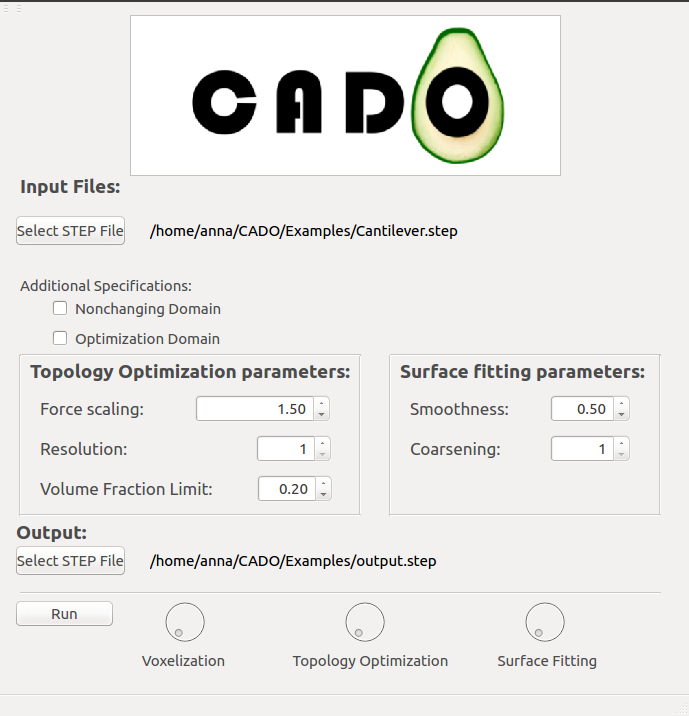
\includegraphics[scale=0.5]{Pictures/CADO_mainWindowParameters.png}
\caption{CADO User Interface showing file input and parameters for topology optimization and surface fitting. During execution of the program, the dials at the bottom indicate progress of the operation}
\label{fig:mainWindowParameters}
\end{figure}
\todointern{Saumi: Add more meat in the caption}
